\begin{comment}
%================================================================
\begin{frame}{Research Teams in DataSense}
%================================================================

  \begin{center}
    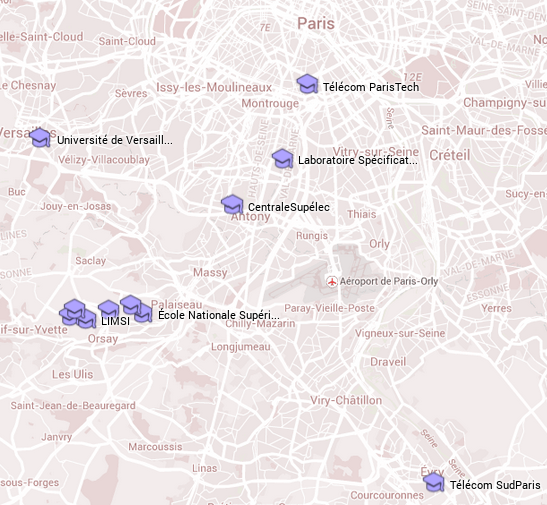
\includegraphics[width=.7\linewidth]{Images/datasense-locations.png}%
    \only<2>{\llap{\raisebox{1cm}{\fbox{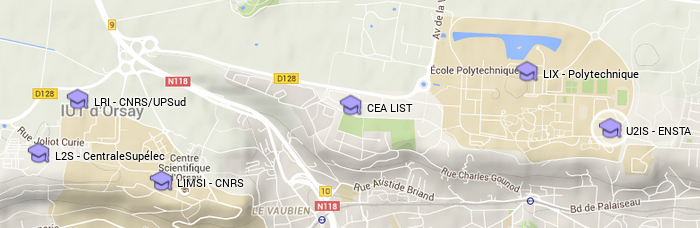
\includegraphics[width=.7\linewidth]{Images/datasense-orsay1.png}}\hspace*{1.5cm}}}}
  \end{center}

\end{frame}
\end{comment}

%================================================================
\begin{frame}{Research Teams in DataSense}

\begin{itemize}
\item \href{http://.david.uvsq.fr/}{DAVID} --- Université Versailles St Quentin
\item \href{http://www.inria.fr/centre/saclay }{Inria Saclay}
\item \href{http://www.l2s.centralesupelec.fr/}{L2S} --- Centrale-Supélec
\item \href{http://www.uvsq.fr/laboratoire-d-informatique-parallelisme-reseaux-algorithmes-distribues-li-parad}{Li-PaRAD} --- Université Versailles St Quentin
\item \href{https://www.limsi.fr/fr/}{LIMSI} --- CNRS – Université Paris-Sud
\item \href{http://www-list.cea.fr/}{LIST} --- CEA
\item \href{http://www.lix.polytechnique.fr/}{LIX} --- École Polytechnique
\item \href{http://lmv.math.cnrs.fr/}{LMV} --- Université Versailles St Quentin
\item \href{http://www.lsv.ens-cachan.fr/}{LSV} --- ENS – Cachan
\item \href{http://www.lri.fr/}{LRI} --- Université Paris-Sud
\item \href{https://www.ltci.telecom-paristech.fr/}{LTCI} --- Télécom Paris-Tech
\item \href{http://www.mics.ecp.fr/}{MICS} --- Ecole Centrale – Paris
\item \href{http://www.samovar.telecom-sudparis.eu/}{SAMOVAR} --- Télécom Paris-Sud
\item \href{http://u2is.ensta-paristech.fr/}{U2IS} --- Université Versailles St Quentin
\end{itemize}
\end{frame}

%%% Local Variables: 
%%% mode: latex
%%% coding: utf-8-unix
%%% ispell-local-dictionary: "english"
%%% TeX-master: "datasense-2016.tex"
%%% fill-column: 9999
%%% End: 
